\documentclass[12pt]{article}

\usepackage{bm}
\usepackage{graphicx}
\usepackage{hyperref}
\usepackage{listings}
\usepackage[top=1in, bottom=1.25in, left=1.25in, right=1.25in]{geometry}

\title{Comparison of sequential and parallel implementation of search algorithm}
\date{2020-11-05}
\author{Bibek Pandey, Mukesh Kumar Pokharel, Prabin Kayastha, Prabin Pathak}

\lstset{frame=tb,
  language=Python,
  aboveskip=3mm,
  belowskip=3mm,
  showstringspaces=false,
  columns=flexible,
  basicstyle={\small\ttfamily},
  numbers=none,
  breaklines=true,
  breakatwhitespace=true,
  tabsize=3
}

\begin{document}

\begin{titlepage}
   \begin{center}
       \vspace*{1cm}

       {\huge Sequential and parallel implementation of linear search algorithm} \\
       \vspace{0.5cm}
       Assignment Report

       \vfill

       By \\
       \vspace{0.5cm}
       Bibek Pandey [\textbf{076mscsk003}]\\
       Mukesh Kumar Pokharel [\textbf{076mscsk006}]\\
       Prabin Kayastha [\textbf{076mscsk007}]\\
       Prabin Pathak [\textbf{076mscsk008}]
       \vspace{1.5cm}

       \vfill

       An assignment presented to \\
       \vspace{0.3cm}
       \textbf{Prof. Dr.\ Subarna Shakya}

       \vspace{1.5cm}
       \textbf{2020 November 05}

   \end{center}
\end{titlepage}

\section*{Problem: parallel and sequential search}
We slightly modified the problem statement to not only find the index of first appearance of the searched number, but also to calculate the total number of appearances 
of the number in the list. This way, all of the array will be traversed and the program does not have to exit when the element is found which reduces complex
communication between the processes.

\section*{Approach 1}
In this approach, we generated numbers in the program itself and passed chunks to corresponding processes to search for a given number. However, there were some issues:
\begin{itemize}
    \item The parallel search ran slower than the sequential search for "not large enough" datasets. Only when the dataset size was large enough (approx. 10 million)  provided expected results.
    \item With large datasets, the copying of the chunks from main process to other spawned process took a lot of memory and hence ran very slow, sometimes even crashing the program itself.
\end{itemize}

\section*{Approach 2}
Here the numbers are generated separately and loaded in a file. With an aim to parallelize the file reading process as well, the numbers are zero-padded so that different
processes can read the chunks in the file easily.

\subsection*{Set up}
100 million random numbers in range (0, 10000000) are generated in a ASCII file, one number in each line and smaller numbers are zero-padded so that every
number is 7-digit long.

\subsection*{Pseudo Code}
\begin{lstlisting}
p <- number of processors
n <- number to search for

declare queue to store processors results

for each processor i, run in parallel:
    read i-th chunk of file
    result:[first_index, total_count] <- search for number in the chunk
    push the result to queue

Now collect results
for each i in 0 to p-1:
    [ind, count] <- result from queue
    accumulate count and compare ind for least index
return accumulated count and first index
\end{lstlisting}

\section*{Result}
We ran the parallel and sequential algorithms in datasets of size 100000,
1000000, 10000000 and 100000000 using 1 to 8 processors. Corresponding speedup vs number of processors plot is shown below.

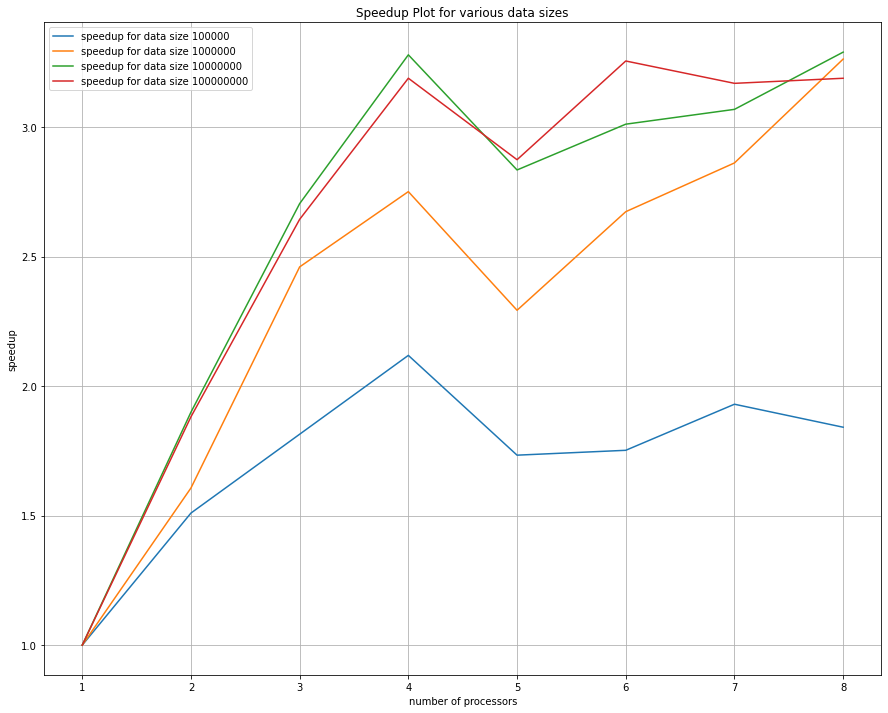
\includegraphics[width=15cm, height=12cm]{speedup-graph}

\section*{Conclusion}
From the graph above we can see the obvious speedup of the search process when multi processors are used.
The speedup monotonically increases upto the point where 4 processors are used. Then strangely enough, for
every dataset size, there is a sudden drop in speedup for 5 processors. The speedup in general again rises
 except for the smallest dataset size. 

It is also important to note that, ignoring the drop of speedup for 5 processors, the speedup tends to be flat afterwards,
conforming to \textbf{Amhdal's Law}.

\section*{Source Code}
The source code is located \href{https://github.com/bewakes/076-mscsk/blob/master/assignments/CS/assignment-Nov-04-2020/search.py}{here}

\section*{Sources}
\begin{itemize}
    \item[-] \href{https://docs.python.org/3.8/library/multiprocessing.html}{Python docs for multiprocessing}
\end{itemize}

\end{document}
